{\bf  We propose here an optimized WFC3-IR snapshot survey designed to find the first ever multiply-imaged supernova (SN), exploiting the magnification power of strong-lensing galaxy clusters and the many multiple-images of different backrgound galaxies each of them offers.}
Exactly fifty years after it was first discussed (Refsdal 1964), thanks to the WFC3 capabilities and the many lensing galaxy clusters recently well-analyzed (e.g. Zitrin et al. 2012a,b, 2013a,b), we have now designed an optimal target list of well-studied efficient lensing clusters, and an obsrvational plan inexpansive in HST time, yielding very good chances of finding several, or at least the long-awaited-for first multiply-imaged SN. Even with a single SN time delay, we will be able to constrain \Ho\ to about 10\% precision, but more importantly, deliver a new, independent and unique test of systematic biases in other time delay measurements, cosmological
probes, and in the lens models themselves.

\medskip
\noindent {\bf Motiviation~~~} The HST archive now holds a deep trove of WFC3-IR imaging on
strong-lensing galaxy clusters at redshifts $z\sim0.2-0.7$.  Thanks to much effort ( Kneib et al., 2004, Smith et al. 2005, Richard et al. 2009, Limousin et al. 2008, Bradac et al. 2008**, as few examples) including a leading role by our group (e.g. in the framework of the CLASH program and beyond; Zitrin et al. 2009a,b; 2011a,b,c; 2012a,b, 2013a,b; Merten et al. 2011; Coe et al. 2012, 2013), unprecedented numbers of multiply-imaged background sources were identified and used to tighly constrain the cluster lens models, enabled by a combination of multi-band imaging by HST (e.g. the CLASH program, PI: Postman), and our light-traces-mass lens modeling technique, which excels in describing cluster lenses with great detail and has the inherent prediction power for finding multiple-images (Broadhurst et al. 2005, Zitrin et al. 2009b).  When a SN inevitably appears within one of these multiply-imaged galaxies, it will of course be multiply-imaged itself. 

\noindent As light from a distant source passes through a galaxy cluster,
strong gravitational lensing causes multiple images to appear to the
observer, separated by a time delay 

\vspace{-5mm}
\hspace{-1.4cm}
\begin{tabular}{p{7cm}r}
% \dt = \frac{\Dl \Ds}{\Dls} ( 1 + z_l ) \phi
{\begin{align}
%\begin{equation}\label{eq:dt}
 %  \dt = \frac{\Dl \Ds}{\Dls} ( 1 + z_l ) \phi
%\end{equation}
  \dt = \frac{(1+z_L)}{c}\frac{\Dl \Ds}{\,\Dls} \phi, \label{eq:dt} \\
\mbox{where}~~ \phi = \frac{1}{2}(\theta-\beta)^2 - \psi(\theta), \label{eq:phi}
\end{align}}
&
\hspace{0.7cm}
\raisebox{-30mm}{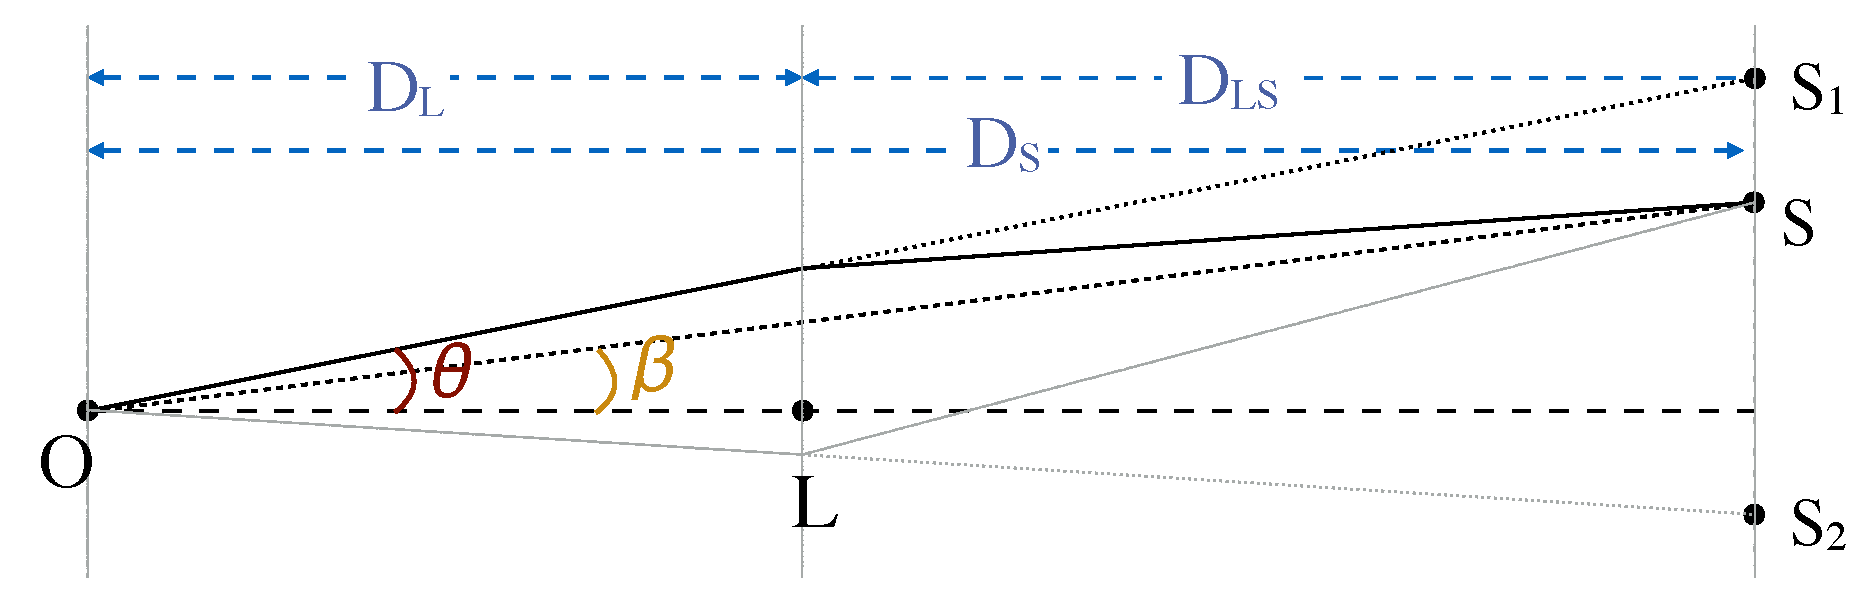
\includegraphics[width=0.52\textwidth]{FIG/lensingGeometry2}}
%\raisebox{-30mm}{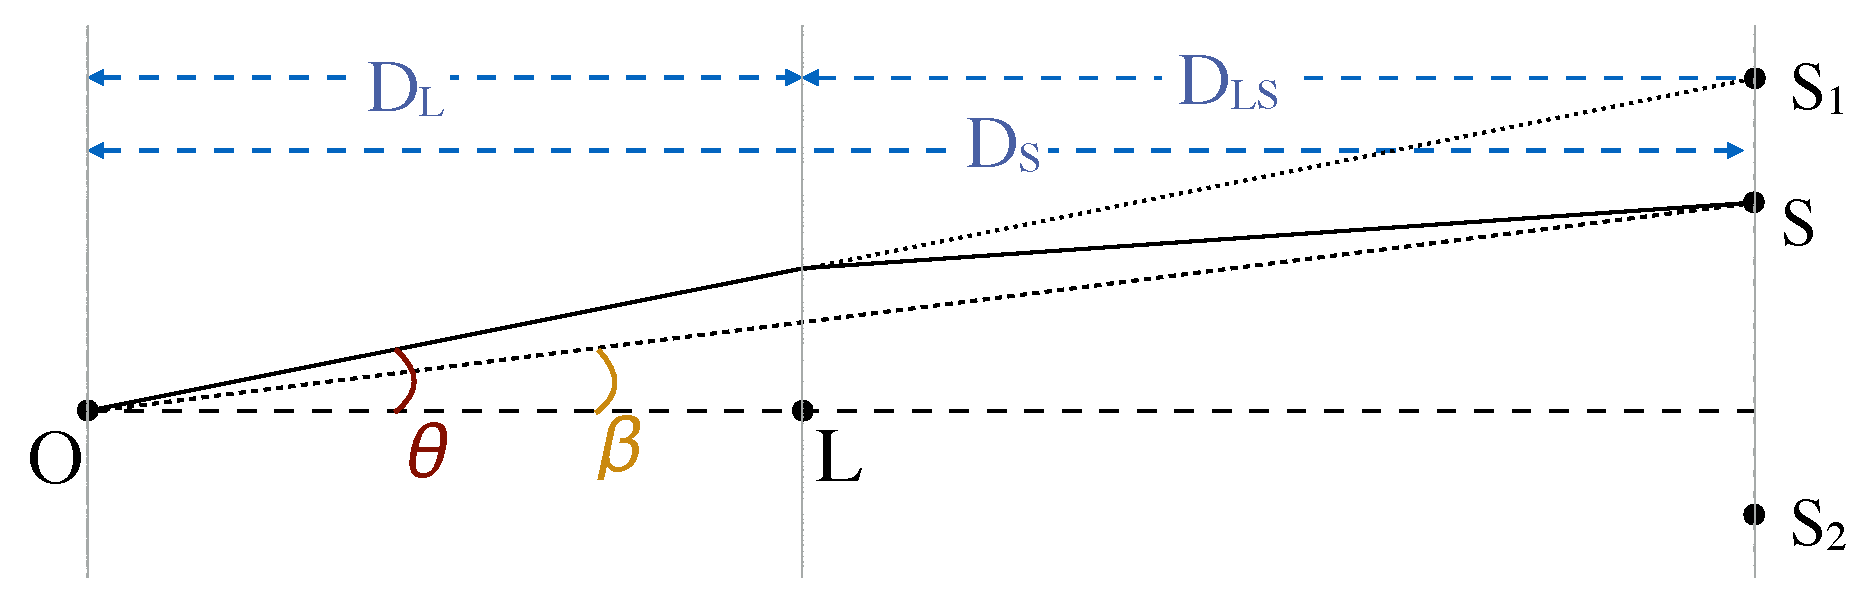
\includegraphics[width=0.5\textwidth]{FIG/lensingGeometry}}
\end{tabular}


\noindent and $z_L$ is the redshift of the lens, while \Dl, \Ds, 
and \Dls\ are angular diamater distances from the observer to the
lens, observer to source, and lens to source, respectively.  In
Eq.~\ref{eq:phi} for the time delay potential  ($\phi$), the first
term gives the geometric delay due to light rays following different
path lengths to the observer, and the second term, $\psi$, is the
relativistic component due to differing values of the gravitational
potential along each path. The distance ratio $\Dl\Ds/\Dls$ in Eq. 1 carries a factor \Ho$^{-1}$, so if the lensing potential $\phi$ is well known,
a time delay measurement provides a direct measurement of the
Hubble constant -- independent of the local distance ladder.  

 \emph{Despite the long-standing prediction, to date, no multiply-imaged SN was found}. The lack of multiply-imaged SNe can be attributed a low number of lenses properly analyzed until recently, and the short visibility window
for any given high-$z$ SN event ($\sim$a few weeks). Only recently were the first few magnified SNe detected behind galaxy clusters: Amanullah et al. ** deteced a magnified SN behind the lensing cluster A1689, and three other magnified SNe were uncovered by us in the CLASH program (Patel et al. 2013/4**, see also Nordin et al. 2013/4**), yet all of these are too far away from the center to be multiply-imaged. 
%It would be almost impossible to detect a multiply-imaged SNe unless a survey is specifically designed to do so. Now, %thanks to the many lensing clusters recently analyzed and many multiply-imaged background galaxies found in them, %we can actually understand what are the best targets to search for multiply-imaged SNe, with minimal HST time %investment, and aided by the capabilities of the WFC3-IR camera. 

\medskip
\noindent {\bf Detecting The First Multiply-Imaged SN~~~} In Cycle 22, HST has just achieved a new capability for the discovery of a multiply-imaged SN. The first key advancement was the
availability of WFC3-IR, which allows HST imaging surveys to capture
high-$z$ SN at the peak of their SED profile in rest-frame optical
bands \citep{Rodney:2012,Jones:2013}.  Ground-based surveys and even
HST/ACS programs have searched for multiply-imaged SN in the past, but
none have had the capability to detect even highly magnified SN at
$z>2$ \citep[e.g.][]{Dawson:2009,Sharon:2010,Sand:2011}.  With
WFC3-IR, \Hubble\ now has access to a much larger survey volume with
each pointing.

A WFC3-IR program targeting massive clusters, such as CLASH or the
Hubble Frontier Fields, could in principal have caught a strongly
lensed SN already.  CLASH, for example, collected
WFC3-IR imaging of 25 clusters over 3 years, but the time separation
between the first and last IR image on any single cluster was
typically only $\sim$40 days, so in practice each cluster only had one
epoch suitable for a lensed SN search rendering serendipiuos detection extremely unlikely. 
However, CLASH and other programs have now provided the second critical
advance: deep IR template imaging of massive clusters from which to
construct difference images for SN discovery. Our snapshot program will capitalize on this rich new treasury, focusing on a carefully-chosen cluster target list (Table~\ref{tab:clusters}). 

In optimizing the target list, one has to take into account the trade-off between the lensing power of a lens and the time-delay, which we have now investigated. Very massive clusters, will generally multiply-lens more background objects, increasing the chances of detecting a SN in one of the few-dozen backrgound galaxies being multiply-imaged. However, very massive clusters will also, on avarage, yield time delays which are hard to measure on a reasonable time scale (can be up to thousands of years), and only a smaller portion of the multiple-image pairs (down to $\sim10-20\%$ following our calculations) would yield desired time delays of a few-months to few-years timescale (allowing for more precise measurements of \dt~and with ample time to prepare for the
appearance of the second image). As a counter-example, galaxy-scale lenses also produce useful time-delays that can be measured on a timescale of days or weeks, but these lenses each comprises typically only one background galaxy and it would take an immense effort to find a multiply-imaged SNe in them. Therefore, optimal targets, as a rule of thumb (i.e. there is also depndence on the exact structure and redshift of the lens), for a timescale of months to few-years time delays, are medium-to-large sized lenses (Einstein radii of roughly $\sim10-30\arcsec$) comprising each few to few-dozen multiply-imaged galaxies.  We have now compiled a list of well-studied clusters, the majority of which are CLASH or Frontier Fields (PI: Lotz) clusters which we have studied in detail, and in which many multiple-images of background galaxies are apparent. For all of these clusters we have in hand state-of-the-art lens models (Zitrin et al., ****, 2014 in prep for the full CLASH sample) which are crucial for the accurate determination of H$_{0}$. Our list contains in total ** lenses spread neatly across the sky, the bulk of which is designed to follow the selection criteria specified above, but supplemented by 2-3 more massive clusters for completeness comprising an order of a hundred multiple images each (Table~\ref{tab:clusters}). 

Time delays can also be measured from other variable sources, such as quasars,
typically lensed by a single foreground galaxy \citep{Jackson:2007}. Among
these, only a handful have time delays measured with particularly high
precision \citep[e.g.][]{Suyu:2010,Suyu:2013}. Additionally, only a few quasars are known to be lensed by \emph{galaxy clusters} (e.g. Ofek \& Maoz 2003, Oguri et al. ** , Dahle et al. 2013). Unlike a multiply-imaged SN which is inherently single-peaked allowing to avoid phase-ambiguity, multiply-imaged quasars can require a long monitoring time for the time-delay to be well measured, albeit this has been done most successfully (Fohlmeister **). Discovering here the first multiply-imaged SNe, will not only enable a complementing and different independent meaure of the time-delay and the Hubble parameter, thus supplying independent tests of crucial systematic biases in other time-delay measueremnts and other cosmological probes, but may also reveal systematics in the lens models themselves hidden otherwise (e.g. Oguri et al. **). These systematics are a crucial factor in current Director's Discretionary Time studies of the high-redshift, magnified Universe such as the Frontier Fields program with HST${^1}$\footnotetext[1]{for which the co-PI A. Zitrin acted as an external lensing-science advisor, and in which we have (PI: Rodney) a program to search for general SNe}, for which the lens-magnification models are key. Finally, if the lensed SN is of Type Ia (a likely prospect), then light curve fitting can provide a luminosity distance measurement with $\sim$8\% precision \citep{Phillips:1993}, and this lensed \SNIa\ could easily
be among the most distant \SNIa\ ever seen.


\medskip
\noindent {\bf The HST Snapshot Search Strategy~~~} To estimate the number of snapshots we need, we start with a
tabulation of the number of known multiply-imaged galaxies in the
fields of our target clusters (Table~\ref{tab:clusters} ** we need to list the number of images, maybe not only the useful fraction?).  This is a
conservative approach, as it is quite possible to detect a
multiply-imaged SN even if the host galaxy is well below the current
detection thresholds for these cluster fields. The total yield of
strongly-lensed SN per snapshot is 
$N_{SN} = SNR_{M} \times M_{gal} \times N_{gal} \times t_{vis}$. 
Here $SNR_M$ is the SN rate per unit mass, $M_{gal}$ is
the average mass of a multiply-imaged galaxy, $N_{gal}$ is the number
of multiply imaged galaxies in the field, and $t_{vis}$ is the length
of time that any given SN is visible to our snapshot survey.  

Most of the lensed systems in our target list are at $z\sim 2$, in an
era near the peak of the cosmic star formation history, so we assume
that our average lensed galaxy is generating SN at a rate similar to
an Sc galaxy in our local universe: $SNR_{M} \sim0.2
(100 \mbox{yr})^{-1} (10^{10} \Msun)^{-1}$ for \SNIa\ and $0.7
(100 \mbox{yr})^{-1} (10^{10} \Msun)^{-1}$ for Type
II \citep{Mannucci:2005}.  We adopt an average stellar mass of
$M_{gal}=10^{10.7} \Msun$ \citep{Tomczak:2013}, and use the census of
multiply-imaged systems in Table~\ref{tab:clusters} to predict an
average of $N_{gal}\sim 35$ lensed galaxy images per
cluster$^{2}$.\footnotetext[2]{Note that we count each separate image of a
multiple-image set except the last one (one cannot measure a time delay
from the last appearance). The time delay between each image is of
order months or years, so each snapshot is essentially observing the
same galaxy at several widely-spaced epochs that can be treated as
independent.}  Using simulated SN light curves in 240 multiply-imaged
galaxies (Figure~\ref{fig:tvis}), we find an average $t_{vis}\sim 30$
days for \SNIa\ and $\sim$20 days for SN II.


With these relatively conservative estimates, we get $N_{SN}\sim
0.1$ SN per snapshot, including both Type Ia and II.  To give this
program a good chance at discovering a strongly lensed SN in Cycle 22,
we request 200 snapshots.  Assuming a realistic snapshot execution
rate of $\sim$30\%, this program should yield a sample of $\sim 6 \pm
4$ SN in one year.  Even if our yield prediction is biased high by a
factor of $\sim$2, we still have a better than 68\% chance to catch at
least one.  Given the intrinsic value of each lensed SN, even just a
single detection will nevertheless be an extraordinary step forward
for time delay cosmography.

Finally, we note that this snapshot program is designed mainly for
discovery. Follow-up observations will come from accompanying GO
program (PI: Strolger), using 12 orbits with ToO observations for immediate
confirmation of a SN candidate and measurement of the light curve.
Sometime in the future, a return campaign to catch the next image
would be needed to complete the time delay measurement, using HST,
ground-based AO systems, or possibly JWST, depending on the length of
the delay.


\begin{table}
\caption{Cluster Target List\label{tab:clusters}}
\begin{tabu}{llllcl}
\toprule
\toprule
Cluster & R.A. & Decl. & z & N$_{im}$ $^*$ & References \\
\midrule
\rowfont{\color{blue}}
Abell 2744\dag & 00:14:23.4 & -30:23:26 & 0.31 & 43  & Merten et al. 2011                                         \\
CL0024         & 00:26:35.0 & +17:09:43 & 0.39 & 20  & Zitrin et al. 2009a                                        \\
El Gordo       & 01:02:52.5 & -49:14:58 & 0.87 & 11  & Zitrin et al. 2013b                                        \\
\rowfont{\color{blue}}
Abell 370\dag  & 02:39:52.8 & -01:34:36 & 0.37 & 36  & Richard et al. 2009, ZFF                                   \\
Abell 383      & 02:48:03.4 & -03:31:44 & 0.19 & 18  & Zitrin et al. 2011b                                        \\
\rowfont{\color{blue}}
MACS0416\dag   & 04:16:08.4 & -24:04:21 & 0.40 & 36  & Zitrin et al. 2013                                         \\
MACS0647       & 06:47:50.3 & +70:14:55 & 0.58 & 20  & Zitrin et al. 2011, Coe et al. 2013                        \\
Bullet-a       & 06:58:37.9 & -55:57:00 & 0.3  & 10  & Bradac et al. **                                           \\
Bullet-b       & 06:58:37.9 & -55:57:00 & 0.3  & 11  & Bradac et al. **                                           \\
MACS0717-a     & 07:17:35.6 & +37:44:44 & 0.55 & 18  & Zitrin et al. 2009b, Limousin et al. 2012, Z14             \\
MACS0717-b     & 07:17:35.6 & +37:44:44 & 0.55 & 18  & Zitrin et al. 2009b, Limousin et al. 2012, Z14             \\
MACS0744       & 07:44:52.8 & +39:27:24 & 0.70 & 14  & Zitrin et al. 2011; 2014 in prep                           \\
Abell 611      & 08:00:56.8 & +36:03:23 & 0.21 & 12  & Newman et al. 2013, Z14                                    \\
\rowfont{\color{blue}}
MACS1149\dag   & 11:49:35.7 & +22:23:55 & 0.54 & 29  & Zitrin  \&  Broadhurst 2009, Zheng et al. 2012             \\
\rowfont{\color{blue}}
MACS1206\dag   & 12:06:12.1 & -08:48:04 & 0.44 & 33  & Ebeling et al. 2009, Zitrin et al. 2012                    \\
\rowfont{\color{blue}}
Abell 1689\dag & 13:11:34.2 & -01:21:56 & 0.19 & 117 & Broadhurst et al. 2005, Coe et al. 2010, Diego et al. 2014 \\
\rowfont{\color{blue}}
Abell 1703\dag & 13:15:03.7 & +51:49:27 & 0.28 & 36  & Limousin et al. 200*, Zitrin et al. 2010                   \\
RXJ1347        & 13:47:31.1 & -11:45:12 & 0.45 & 14  & K\"ohlinger \&  Schmidt 2014                               \\
MS1358         & 13:59:48.7 & +62:30:48 & 0.33 & 13  & Zitrin et al. 2011c                                        \\
Abell 1835     & 14:01:02.0 & +02:52:45 & 0.25 & 17  & Richard et al. 2010, Morandi et al. 2012                   \\
Abell 2218     & 16:35:54.0 & +66:13:00 & 0.18 & 18  & Kneib et al. 2004                                          \\
Abell 2261     & 17:22:27.2 & +32:07:57 & 0.22 & 18  & Coe et al. 2012                                            \\
MACS1931       & 19:31:49.6 & -26:34:32 & 0.35 & 10  & Z14                                                        \\
MACS2129       & 21:29:26.1 & -07:41:28 & 0.57 & 14  & Zitrin et al. 2011; Z14                                    \\
\rowfont{\color{blue}}
RXJ2248\dag    & 22:48:44.0 & -44:31:51 & 0.35 & 28  & Monna et al. 2013                                          \\
\bottomrule
% MACS0329   & 03:29:41.6 & -02:11:46 & 0.45 & 11 & Zitrin et al. 2012, Z14                       \\
% MACS0451   & 04:51:54.6 & +00:06:17 & 0.43 & 11                                                 \\
% MACS0454   & 04:54:11.1 & -03:00:53 & 0.54 & 11 & Zitrin et al. 2011                            \\
% CL1226     & 12:26:58.2 & +33:32:48 & 0.89 & 11 & Z14                                           \\
% MACS1423   & 14:23:48.3 & +24:04:47 & 0.54 & 11 & Limousin et al. 2010, Zitrin et al. 2011, Z14 \\
% MACS1720   & 17:20:16.8 & +35:36:26 & 0.39 & 11 & Z14                                           \\
% Abell 2390 & 21:53:55.8 & +17:43:34 & 0.23 & 7  & Frye et al. 1998                              \\
% MS2137     & 21:40:15.2 & -23:39:40 & 0.31 & 7  & Newman et al. 2013, Z14                       \\
% RXJ2129    & 21:29:40.0 & +00:05:21 & 0.23 & 9  & Richard et al. 2010, Z14                      \\
%\enddata
 \multicolumn{6}{p{\textwidth}}{* Approximate number of known strongly-lensed galaxy images
   within the WFC3-IR FOV, counting all instances of each lensed galaxy
   except the last (i.e. all independent lensed galaxy images that
   could deliver a SN time delay measurement).}\\
 \multicolumn{6}{p{\textwidth}}{ \textcolor{blue}{$\dagger$ Primary targets.} We will allocate more
   snapshots to these clusters that have especially strong lenses with
   many multiply-imaged galaxies and particularly good lens models.
   The unweighted average $N_{im}$ is $\sim$25, but we expect this
   weighted snapshot allocation to result in an actual mean of
   $N_{im}\sim 35$.}\\
%\tablenotetext{**}{ Key or latest references for the multiple image
%  compilation in each cluster. Z14 stands for ``Zitrin et al. 2014 in
%  prep" is a soon to be public paper describing our high-end mass
%  models already available online for the community, and multiple
%  images, for all 25 CLASH clusters. ``ZFF" refers to the internal
%  list of the Frontier Fields map making groups, for which Co-PI
%  Zitrin has contributed significantly for revising the multiple
%  images.}
\end{tabu}
\end{table}


%\insertfig{FIG/lightcurves.pdf}{ \label{fig:lightcurves} Lensed SN
%    light curves }

\insertfig{FIG/tvis_muz_20min.pdf}{\label{fig:tvis} 
Visibility time contours in the redshift-magnification plane. Using
simulated light curves of an average lensed Type Ia SN, we have
measured the expected visibility window (a.k.a the control time): the
number of days that the SN is above our detection threshold for a 20-minute
snapshot.  Solid lines plot contours of constant visibility time in
the $z-\mu$ plane at $t_{vis}=$100, 50, and 10 days.  Grey points mark
the measured magnifications and redshifts for 50 strongly-lensed
galaxy images from three of our primary cluster targets. }




